\documentclass[11pt]{article}
\usepackage[tmargin=1in,bmargin=1in,lmargin=1in,rmargin=1in]{geometry}
\usepackage{parskip}
\usepackage{mypackagesv2}

\title{Deliverable 1} 
\author{Jadon Tsai $|$ Jeffery Tian $|$ Pranav Upreti}
\everymath{\displaystyle}

\begin{document}
\captionsetup[figure]{labelfont={it},name={Figure},labelsep=colon} 
\maketitle
\section{Introduction and Assumptions}
This report calculates the Shear Force Diagram, Bending Moment Diagram, FOS against flexural tension failure and flexural compression failure for a beam specified by Design 0. Our calculations assume that (i) the load is centered on the bridge and (ii) is loaded according Load Case 2 shown in \cref{fig:loadingDiagram}. 

We follow the same sign convention used in class. All values are rounded to slide rule precision in the final calculation. 
\begin{figure}[H]
\centering
\begin{tikzpicture}
    % define coordinates
    \point{start}{0}{0};
    \point{end}{12}{0};
    % load coordinates;
    \point{l1}{1.72}{0};
    \point{l2}{3.48}{0};
    \point{l3}{5.12}{0};
    \point{l4}{6.88}{0};
    \point{l5}{8.52}{0};
    \point{l6}{10.28}{0};
    % specify beam location;
    \beam{2}{start}{end}[1][1];
    % specify support locations;
    \support{1}{start} % pin;
    \support{2}{end} % roller;
    % specify point loads;
    \load{1}{l1}[90];
    \load{1}{l2}[90];
    \load{1}{l3}[90];
    \load{1}{l4}[90];
    \load{1}{l5}[90];
    \load{1}{l6}[90];
    % label point loads;
    \notation{1}{l1}{67.5 KN}[above=12.5mm];
    \notation{1}{l2}{67.5 KN}[above=12.5mm];
    \notation{1}{l3}{67.5 KN}[above=12.5mm];
    \notation{1}{l4}{67.5 KN}[above=12.5mm];
    \notation{1}{l5}{91 KN}[above=12.5mm];
    \notation{1}{l6}{91 KN}[above=12.5mm];
    % dimension beam;
    \dimensioning{1}{start}{l1}{-1.45}[172 mm];
    \dimensioning{1}{l1}{l2}{-1.45}[176 mm];
    \dimensioning{1}{l2}{l3}{-1.45}[164 mm];
    \dimensioning{1}{l3}{l4}{-1.45}[176 mm];
    \dimensioning{1}{l4}{l5}{-1.45}[164 mm];
    \dimensioning{1}{l5}{l6}{-1.45}[176 mm];
    \dimensioning{1}{l6}{end}{-1.45}[172 mm];
\end{tikzpicture}
\caption{Base case loading diagram for load case 2}
\label{fig:loadingDiagram}
\end{figure}
To quicken calculations, we wrote a Python script that we validated in Appendix A. % we can probably remove this
\section{Centered Load Case 2 - Base Case}
\subsection{SFD and BMD}
\begin{figure}[H]
\centering
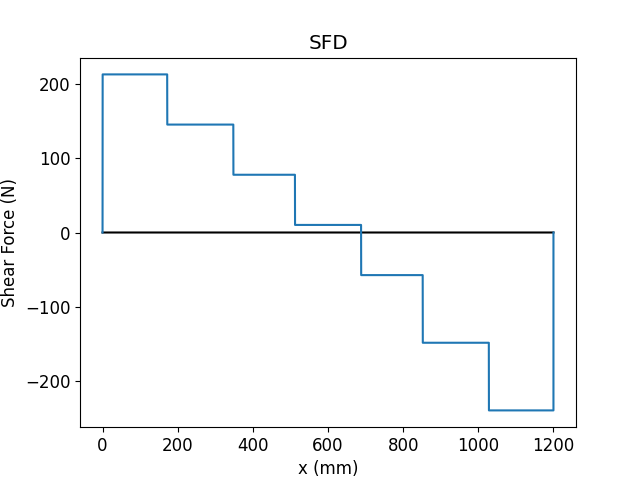
\includegraphics[scale=0.7]{SFDv2.png} 
\end{figure}
\textbf{Maximum positive shear:} 213 N $|$ \textbf{Maximum negative shear:} 239 N 
\begin{figure}[H]
\centering
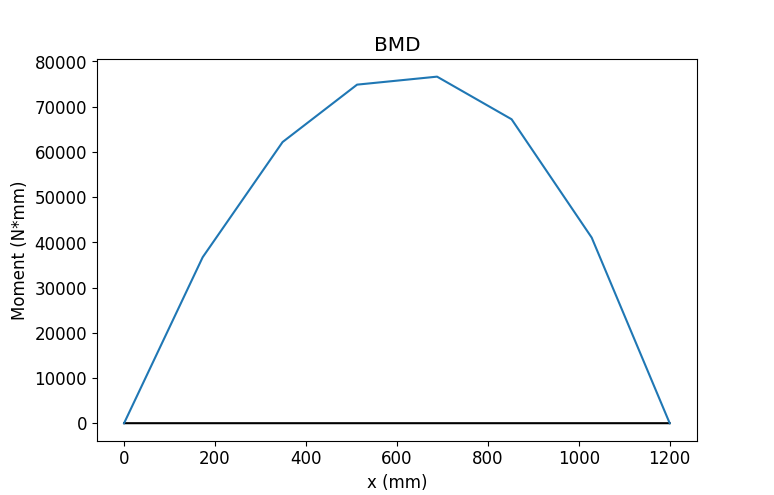
\includegraphics[scale=0.7]{BMDv2.png} 
\end{figure}
\textbf{Maximum moment:} 76666.1 N mm
\section{Determining the F.O.S.}
We can calculate the maximum flexural tension and compressive forces using the maximum bending moment from the diagram with the relation $\sigma = \text{F.O.S.} \frac{M_{\text{max}}(y-\bar{y})}{I}$ or  $\text{F.O.S.} = \frac{\sigma I}{M_{\text{max}}|y-\bar{y}|}$.

\noindent\rule[7pt]{\linewidth}{0.4pt}
$I = 418352.21$ mm$^4$ and $\bar{y} = 41.43$ mm, calculated using a Python script 

For the maximum flexural compressive strength in the beam, $\sigma = 6$ MPa:
\begin{align*}
\text{F.O.S. } &= \frac{\sigma_c I}{M_\text{max}|y-\bar{y}|}\\
               &= \frac{(6 \text{ MPa})(418352.21 \text{ mm}^4)}{(76666.1 \text{ N mm})(76.27\text{ mm}-41.43 \text { mm})} \\
               &= 0.940 \\
\Aboxed{\therefore \text{F.O.S. in compression}               &= 0.940} 
\end{align*}
And for the maximum flexural tensile force:
\begin{align*}
\text{F.O.S. } &= \frac{\sigma_t I}{M_\text{max}|y-\bar{y}|}\\
               &= \frac{(30 \text{ MPa})(418352.21 \text{ mm}^4)}{(76666.1 \text{ N mm})(76.27\text{ mm}-41.43 \text { mm})} \\
\Aboxed{\therefore \text{F.O.S. in tension}               &= 3.95} 
\end{align*}

\section{Appendix A: Validating our Python Script}
The Python script we wrote is linked \href{https://github.com/epsilon-naut/CIV102-Bridge-Project}{here}. \newline
\textbf{Calculating $\bar{\bf y}$:}
\begin{align*}
    \bar{y} &= \frac{\sum_{i=1}^{N}A_iy_i} {\sum_{i=1}^{N}A_i} \\
    &= \frac{100(1.27)(75+\nicefrac{1.27}{2}) + (5+1.27)(1.27)(74.365)\times 2 + 1.27(73.73)(36.865)\times 2 + (80-1.27(2))(0.635)}{(100)(1.27)+(5+1.27)(1.27)\times 2 + 1.27(75-1.27)\times 2 + (80-2.54)(1.27)} \\
    &= 41.43 \text{ mm (\textit{2 d.p.})}
\end{align*}
This matches our code output. \newline
\textbf{Calculating $\bar{\bf y}$:}
\begin{align*}
    I &= \sum_{i=1}^NI_i + \sum_{i=1}^{N}A_iy_i^2 \\
      &= \frac{100(1.27)^3}{12} + \frac{(5+1.27)(1.27)^3}{12}\times 2 + \frac{1.27(73.73)^3}{12}\times 2 + \frac{(80-2.54)(1.27)^3}{12} \\
      &\hspace{40pt} + [(41.43 - (75 + \nicefrac{1.27}{2}]^2(1.27)(100) + [(41.43 - (75 - \nicefrac{1.27}{2}]^2(5+1.27)(1.27)\times 2 \\
      &\hspace{40pt}+ [(41.43 - 36.865]^2(75-1.27)(1.27)\times 2 + [41.43 - 0.635]^2(80-2.54)(1.27) \\
      &= 418352.21 \text{ mm$^4$\textit{(2 d.p.)}}
\end{align*}
This matches our code output.


\end{document}